\documentclass[]{article}
\usepackage{graphicx}
\graphicspath{ {./images/} }

%opening
\title{A simple CNN to clasify CIFAR-10 dataset based on VGG Architecture}
\author{Frank Acquaye}

\begin{document}

\maketitle

\begin{abstract}
This document describes an architectural design in solving the classification challenge of CIFAR-10. The proposed model achieves an accuracy above 0.77 on validation data-set.
\end{abstract}

\section{Model Description}
Owing to the understandable simplicity of the VGG architecture, this architecture was adopted in an attempt to solve the CIFAR-10 classification challenge. 

The chosen architecture comprised primarily of a VGG Block. A VGG block consists of:
\begin{itemize}
	\item A Convolutional layer with a relu activation function
	\item A convolutional layer with a relu activation function
	\item A maxpooling layer
\end{itemize}

These blocks were stacked until a desired accuracy of about 70\% was obtained. This accuracy was obtained after stacking 3 VGG blocks. A 4th VGG block was added but did not seem to improve the performance as much.

The optimizer used was Adam optimizer.
Dropout and Image augmentation were used to develop the final model.

\section{Lessons Learnt}
\begin{itemize}
	\item Although the assignment clearly stated that changes should be made incrementally, this lesson was learnt the hard way. Since huge changes were introduced at some point leading to the deterioration of accuracy. A new model needed to be created from scratch since the offending change was not easily recognized.
	\item In order to obtain a descent accuracy, it involves a lot of experimentation with the architecture
\end{itemize}

\section{Final Model}
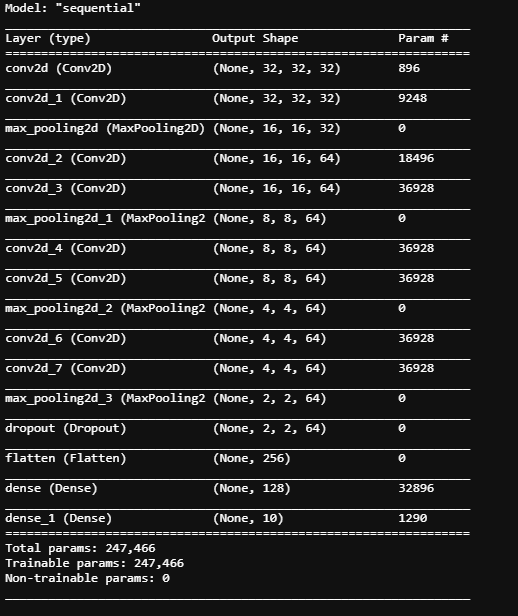
\includegraphics{final_model}


\end{document}
